% Options for packages loaded elsewhere
\PassOptionsToPackage{unicode}{hyperref}
\PassOptionsToPackage{hyphens}{url}
%
\documentclass[
  10pt,
]{article}
\usepackage{lmodern}
\usepackage{amssymb,amsmath}
\usepackage{ifxetex,ifluatex}
\ifnum 0\ifxetex 1\fi\ifluatex 1\fi=0 % if pdftex
  \usepackage[T1]{fontenc}
  \usepackage[utf8]{inputenc}
  \usepackage{textcomp} % provide euro and other symbols
\else % if luatex or xetex
  \usepackage{unicode-math}
  \defaultfontfeatures{Scale=MatchLowercase}
  \defaultfontfeatures[\rmfamily]{Ligatures=TeX,Scale=1}
\fi
% Use upquote if available, for straight quotes in verbatim environments
\IfFileExists{upquote.sty}{\usepackage{upquote}}{}
\IfFileExists{microtype.sty}{% use microtype if available
  \usepackage[]{microtype}
  \UseMicrotypeSet[protrusion]{basicmath} % disable protrusion for tt fonts
}{}
\makeatletter
\@ifundefined{KOMAClassName}{% if non-KOMA class
  \IfFileExists{parskip.sty}{%
    \usepackage{parskip}
  }{% else
    \setlength{\parindent}{0pt}
    \setlength{\parskip}{6pt plus 2pt minus 1pt}}
}{% if KOMA class
  \KOMAoptions{parskip=half}}
\makeatother
\usepackage{xcolor}
\IfFileExists{xurl.sty}{\usepackage{xurl}}{} % add URL line breaks if available
\IfFileExists{bookmark.sty}{\usepackage{bookmark}}{\usepackage{hyperref}}
\hypersetup{
  pdftitle={Welcome Home --- Now Vote!},
  pdfauthor={Kevin Morris},
  hidelinks,
  pdfcreator={LaTeX via pandoc}}
\urlstyle{same} % disable monospaced font for URLs
\usepackage[margin=1in]{geometry}
\usepackage{longtable,booktabs}
% Correct order of tables after \paragraph or \subparagraph
\usepackage{etoolbox}
\makeatletter
\patchcmd\longtable{\par}{\if@noskipsec\mbox{}\fi\par}{}{}
\makeatother
% Allow footnotes in longtable head/foot
\IfFileExists{footnotehyper.sty}{\usepackage{footnotehyper}}{\usepackage{footnote}}
\makesavenoteenv{longtable}
\usepackage{graphicx}
\makeatletter
\def\maxwidth{\ifdim\Gin@nat@width>\linewidth\linewidth\else\Gin@nat@width\fi}
\def\maxheight{\ifdim\Gin@nat@height>\textheight\textheight\else\Gin@nat@height\fi}
\makeatother
% Scale images if necessary, so that they will not overflow the page
% margins by default, and it is still possible to overwrite the defaults
% using explicit options in \includegraphics[width, height, ...]{}
\setkeys{Gin}{width=\maxwidth,height=\maxheight,keepaspectratio}
% Set default figure placement to htbp
\makeatletter
\def\fps@figure{htbp}
\makeatother
\setlength{\emergencystretch}{3em} % prevent overfull lines
\providecommand{\tightlist}{%
  \setlength{\itemsep}{0pt}\setlength{\parskip}{0pt}}
\setcounter{secnumdepth}{5}
\usepackage{rotating}
\newcommand{\beginsupplement}{\setcounter{table}{0}  \renewcommand{\thetable}{A\arabic{table}} \setcounter{figure}{0} \renewcommand{\thefigure}{A\arabic{figure}}}
\usepackage{setspace}
\usepackage{booktabs}
\usepackage{longtable}
\usepackage{array}
\usepackage{multirow}
\usepackage{wrapfig}
\usepackage{float}
\usepackage{colortbl}
\usepackage{pdflscape}
\usepackage{tabu}
\usepackage{threeparttable}
\usepackage{threeparttablex}
\usepackage[normalem]{ulem}
\usepackage{makecell}
\usepackage{xcolor}
\newlength{\cslhangindent}
\setlength{\cslhangindent}{1.5em}
\newenvironment{cslreferences}%
  {\setlength{\parindent}{0pt}%
  \everypar{\setlength{\hangindent}{\cslhangindent}}\ignorespaces}%
  {\par}

\title{Welcome Home --- Now Vote!\thanks{Prepared for the 2020 Annual Meeting of the Midwest Political Science Association. The author thanks Jacob Faber, Jeff Manza, Myrna Pérez, Ariel White, and Peter Miller for their comments on this project. All errors are my responsibility.}}
\usepackage{etoolbox}
\makeatletter
\providecommand{\subtitle}[1]{% add subtitle to \maketitle
  \apptocmd{\@title}{\par {\large #1 \par}}{}{}
}
\makeatother
\subtitle{Voting Rights Restoration and Post-Supervision Participation}
\author{Kevin Morris\footnote{Researcher, Brennan Center for Justice at NYU School of Law, 120 Broadway Ste 1750, New York, NY 10271 (\href{mailto:kevin.morris@nyu.edu}{\nolinkurl{kevin.morris@nyu.edu}})}}
\date{July 06, 2020
\linebreak
\linebreak
\linebreak
\linebreak
Word Count: 9,596}

\begin{document}
\maketitle
\begin{abstract}
This paper presents causal estimates of the effect of voting rights restoration prior to discharge from parole on post-supervision participation. In 2018, New York State began restoring voting rights to parolees, after previously restoring voting rights only at the completion of parole. By leveraging randomness in parole discharge date, I interrogate whether restoring voting rights to formerly incarcerated individuals while still on parole increases their post-supervision propensity to cast a ballot. I demonstrate that in-person rights restoration prior to parole discharge significantly increased turnout. This group-level effect, however, masks race-specific effects. Although rights restoration prior to parole discharge effectively doubled turnout among white former parolees, it had no measurable effect on the turnout of non-white former parolees. This raises serious questions about how rights restoration programs are implemented, and how incarceration might differently structure Black Americans' view of the democratic process.
\end{abstract}

\pagenumbering{gobble}
\pagebreak
\doublespacing

\pagenumbering{arabic}

\hypertarget{introduction}{%
\section*{Introduction}\label{introduction}}
\addcontentsline{toc}{section}{Introduction}

In all but two states (Maine and Vermont), felony disenfranchisement laws mean that American citizens convicted of felony offenses lose the right to vote for at least some period of time. In some states, such as Oregon and Massachusetts, individuals lose that right only for the period in which they are actively incarcerated. Iowa stands alone at the other end of the spectrum, where felony convictions result in lifelong disenfranchisement unless a returned citizen receives an individual pardon from the state's governor (Justice \protect\hyperlink{ref-bcj_laws}{2019}). This variation in laws arises from language in the Fourteenth Amendment which allows states to revoke individuals' voting rights ``for participation in rebellion, or other crime.'' The definition of ``other crime,'' left so vague in the Constitution, is now generally used by states to disenfranchise citizens for any felony offense. The Supreme Court, in cases such as \emph{Richardson v. Ramirez} (1974), has upheld this practice. Collectively, these laws disenfranchise as many as 4.7 million American citizens. Of these, the majority are no longer incarcerated (Uggen, Larson, and Shannon \protect\hyperlink{ref-sentencing_2016}{2016}).\footnote{The figures reported in Uggen, Larson, and Shannon (\protect\hyperlink{ref-sentencing_2016}{2016}) have been adjusted to reflect the impact of Amendment 4 in Florida.}

There is some evidence that incarceration continues to structure political participation even after an individual is no longer legally disenfranchised. As previous literature has established, interactions with the criminal justice system leaves residents less likely to vote in the future (White \protect\hyperlink{ref-White2019}{2019}; but see Gerber et al. \protect\hyperlink{ref-Gerber2017}{2017}). As Burch (\protect\hyperlink{ref-Burch2011}{2011}) and others have shown, moreover, turnout rates among the formerly incarcerated are extremely low. Formal disenfranchisement policy, the literature has made clear, is just one piece of an interlocking system that serves to disenfranchise minority and marginalized voters. The incarcerated population is drawn from a pool of individuals unlikely to vote even prior to their incarceration. To address only the formal laws contributing to disenfranchisement without also interrogating efforts to boost post-supervision participation risks leaving much of the system of effective disenfranchisement undisturbed. New York State offers us the opportunity to test how the timing and method of the re-instation of voting rights structures post-supervision participation.

Prior to 2018, New Yorkers convicted of felony offenses and sentenced to prison were disenfranchised until they had completed all terms of their sentence --- their period of incarceration as well as any parole term. For New Yorkers on life parole or sentenced to life in prison, this law resulted in effective lifetime disenfranchisement. New Yorkers sentenced to felony probation, on the other hand, did not lose their voting rights.

In the spring of 2018,\footnote{Although the executive order was signed on April 18\textsuperscript{th}, it did not go into effect until May 18\textsuperscript{th}.} Governor Andrew Cuomo signed Executive Order 181 which effectively ended the disenfranchisement of New Yorkers on parole. Such a move of course directly re-enfranchised individuals who were still on parole on election day. The change in policy is also perhaps beneficial for felony probationers: despite the fact that probationers do not formally lose their voting rights, there is evidence that confusion around the law contributes to \emph{de facto} disenfranchisement among probationers (Drucker and Barreras \protect\hyperlink{ref-Drucker2005}{2005}).

The executive order may also have increased the political participation of \emph{formerly} disenfranchised individuals. Prior to the policy change, formerly incarcerated individuals had their voting rights restored automatically upon the completion of their parole term. New York's correction code provides no more guidance other than that ``upon a person's discharge from community supervision, the department shall notify such person of his or her right to vote and provide such person with a form of application for voter registration'' (Section 75 of the New York State Correction Law). Shortly after the implementation of the executive order, Acting Deputy Commissioner for Community Supervision Ana Enright sent a memorandum to New York State parole officers detailing the Department of Corrections' new approach.\footnote{Link: \url{https://nyassembly.gov/member_files/139/webdocs/82103.pdf}} The memorandum directs all parole officers to present parolees with voter registration forms and to explain their purpose. Parole officers are instructed to offer any assistance needed, including help filling out the registration form. In addition to these directives, the memorandum communicates that voter registration is to receive ``high priority attention,'' and it separately calls the program ``a \textbf{priority} initiative'' {[}emphasis in the original{]}. Thus, the executive order demands not only that re-enfranchised individuals receive in-person notification of their voting rights, but also that parole officers prioritize their registration.

In the analysis below, I examine the effect of Executive Order 181 on individuals who finished parole before October 10th, 2018 (the registration deadline for 2018). I exclude individuals who were still on parole and could only vote because of the policy change in order to unpack how the mechanisms of rights restoration can shape turnout.

By examining the effect of rights restoration in the context of a personal relationship with a parole officer against a status quo in which formerly incarcerated individuals were informed of their eligibility through the mail, Executive Order 181 offers us the opportunity to build on existing research. Do these human interactions repair damage done to the formerly incarcerated individual's relationship to the state? Or do parole officers exhibit biases against their stewards, making them ineffective or uneven conduits for restoration?

\hypertarget{notification-re-enfranchisement-and-turnout}{%
\section*{Notification, Re-enfranchisement, and Turnout}\label{notification-re-enfranchisement-and-turnout}}
\addcontentsline{toc}{section}{Notification, Re-enfranchisement, and Turnout}

Whether --- and to what extent --- incarceration causes lower turnout among citizens is the subject of some debate in the literature. Gerber et al. (\protect\hyperlink{ref-Gerber2017}{2017}), for instance, argues that prison does not materially impact post-incarceration turnout, though White (\protect\hyperlink{ref-White2019}{2019}) finds that jail time can decrease the future turnout of misdemeanants. Regardless of the causal impact of incarceration on turnout, however, it is well established that formerly incarcerated individuals turn out at relatively low rates (see, for instance, Burch (\protect\hyperlink{ref-Burch2011}{2011})).

Regardless of whether incarceration reduces turnout, the state has a unique opportunity to craft policies that will impact individuals under formal supervision. Even if incarceration does not lead to lower turnout, policies targeting individuals caught up in the criminal justice system might still be effective at increasing their turnout.

Formerly convicted individuals are very often confused about their eligibility to vote (Drucker and Barreras \protect\hyperlink{ref-Drucker2005}{2005}; Manza and Uggen \protect\hyperlink{ref-locked_out}{2008}). Some research indicates that dispelling misinformation boosts turnout among the formerly disenfranchised. Meredith and Morse (\protect\hyperlink{ref-Meredith2015}{2015}) examines the impact of ending permanent disenfranchisement in Iowa. Prior to 2005 (and after 2011), individuals with felony convictions were permanently disenfranchised unless they submitted an application to the governor. Executive Order 42 eliminated this requirement, instead re-enfranchising individuals automatically upon sentence completion. Although all formerly disenfranchised individuals were re-enfranchised upon the signing of the Executive Order, not all re-enfranchised individuals were informed of their change in status. Meredith and Morse (\protect\hyperlink{ref-Meredith2015}{2015}) leverages differences in notification to test whether the notification increased turnout, finding a strong positive effect. Meredith and Morse (\protect\hyperlink{ref-Meredith2013}{2013}), on the other hand, examines states where so-called notification laws went into effect. Although rules about eligibility did not change in these states, new policies required Departments of Corrections to notify formerly disenfranchised individuals of their re-instated voting rights. Meredith and Morse (\protect\hyperlink{ref-Meredith2013}{2013}) finds no effect on turnout from notification in the absence of eligibility changes.

Gerber et al. (\protect\hyperlink{ref-Gerber2015}{2015}) built on the quasi-experimental design of Meredith and Morse (\protect\hyperlink{ref-Meredith2015}{2015}), conducting a field experiment in Connecticut in advance of the 2012 presidential election. In their field experiment, some formerly convicted (but eligible) residents were reminded of their eligibility; others were not. Like Meredith and Morse (\protect\hyperlink{ref-Meredith2015}{2015}), they find evidence that these reminders successfully increased turnout. ``Whatever the participatory consequences of incarceration,'' they conclude, ``they are not in large part impossible to overcome'' (924). Even if incarceration does not decrease individuals' propensity to vote, there is reason to believe that reminding formerly incarcerated individuals of their rights increases participation.

Meredith and Morse (\protect\hyperlink{ref-Meredith2015}{2015}) and Gerber et al. (\protect\hyperlink{ref-Gerber2015}{2015}) provide valuable insight into mechanisms that can increase the turnout of formerly disenfranchised individuals. Nevertheless, the research to date has examined the effect of mail notification on post-supervision turnout. In the case of New York State, formerly incarcerated individuals were already informed of their voting rights through the mail when they finished their sentence prior to the executive order. In other words, the treatment identified in past research is here incorporated into the status quo, or control, condition. This study therefore tests not the efficacy of notification laws but rather whether in-person restoration prior to discharge increases turnout above-and-beyond any increase associated with mail notification.

There is reason to believe that some of the negative treatment effects of incarceration arise from the very nature of person-to-person relationships in the criminal justice system. Lerman and Weaver (\protect\hyperlink{ref-Lerman2014}{2014}) argues that contact with the criminal justice system can uniquely structure democratic participation more than other types of government contact. ``It may also be,'' they write, ``that social benefits {[}arising from non-criminal justice contact with the state{]} are less visible to citizens because they often occur through the mail, rather than through personal contact with government agencies or officials, making it easier to disconnect social benefits from government and the political system'' (93). Because Executive Order 181 operates \emph{not} through the mail but rather through ``personal contact with government\ldots{} officials,'' its effects may differ from the mail notification programs. The social benefits (restoration of voting rights) might be communicated more effectively and in ways that improve the formerly incarcerated individuals' opinions of their democratic state, thus increasing turnout further.

Of course, reliance on a human-mediated system to deliver social benefits poses potential practical and scientific complications. A notification sent in the mail is a binary treatment: the letter was either sent or not sent. Communicating the restoration of voting rights through human interaction means that the treatment might vary by individuals: if parolees have a warm relationship with their parole officer, they may be strongly encouraged to register and participate. On the other hand, if parole officers are biased against their parolees (due either to racial hostility, personal dislike, or expected partisan affiliation) they may not provide any effective treatment at all. Thus, while the communication of voting rights restoration in the context of a personal relationship has the potential to deliver much larger benefits, it also opens the door to potential discrepancies in treatment.

I expect that restoring voting rights while an individual is still on parole increases that individual's later propensity to vote substantially. This increase will operate through two mechanisms: as the previous literature has established, notification of voting rights can increase turnout, and being informed by a parole officer likely leaves a former parolee more sure of her voting rights than a letter in the mail. Secondly, the interpersonal nature of the parolee-parole officer relationship is expected to more effectively repair (some of) the damage done to the former parolees interpretation of the state. Individual, in-person invitations to rejoin the body politic are likely effective.

\hypertarget{data}{%
\section*{Data}\label{data}}
\addcontentsline{toc}{section}{Data}

\hypertarget{criminal-justice-data}{%
\subsection*{Criminal Justice Data}\label{criminal-justice-data}}
\addcontentsline{toc}{subsection}{Criminal Justice Data}

The criminal justice dataset comes from a public records request filed by the author to obtain individual-level incarceration and parole records for individuals sentenced to incarceration in New York State since 1990. The data includes a host of information, including: first, middle, and last name; date of birth; class of offense; incarceration start and end dates; dates of parole; county of commitment; and others. This analysis is limited to individuals incarcerated for felony offenses. Individuals convicted of misdemeanors are not disenfranchised in New York State. These data come from the New York State Department of Corrections and Community Supervision (NYSDOCCS). These data are used to determine when individuals were incarcerated or on parole, when they finished their parole supervision, and demographic information such as age and race.

Following Executive Order 181, the Department of Corrections and Community Supervision began indicating on their online Parolee Lookup Tool whether a parolee had her voting rights restored. By using the identification number provided from the parolee public records request and this website, I was able to identify individuals who had their voting rights restored.\footnote{Not all parolees listed in the public records request data are included in the lookup tool. Roughly 1 percent of former parolees are not in the online lookup.} There were 3,093 individuals who were discharged from parole before the registration deadline whose rights were restored while still under supervision. Roughly 1,200 individuals who were discharged between the effective date of the executive order and the registration deadline did not have voting rights restored, due largely to their status as noncitizens.

\hypertarget{voter-file-data}{%
\subsection*{Voter File Data}\label{voter-file-data}}
\addcontentsline{toc}{subsection}{Voter File Data}

Most states in the United States are required to maintain files with information on all registered voters. In New York, this information is publicly available from the Board of Elections. It includes information on all registered voters, including: first, middle, and last name; date of birth; vote history; and other information. The New York State Voter File also includes information on voters who were previously registered but have since been purged, either because they moved, died, or were incarcerated for a felony offense. I use a snapshot of the registered voter file from March 3\textsuperscript{rd}, 2019.

\hypertarget{matching}{%
\subsection*{Matching}\label{matching}}
\addcontentsline{toc}{subsection}{Matching}

Turnout in the 2018 midterm election is estimated by matching the parole records with the registered voter file. I match individuals in each dataset using first name, middle name, last name, and date of birth. To be considered a ``match,'' records must have the exact same birth date. The first and last names must also be exact matches (conditional on the adjustments discussed below). Middle names must match exactly as well, except for if one record has only a middle initial, which is allowed to match to a full middle name in the other set of records.

I adopt the test developed in Meredith and Morse (\protect\hyperlink{ref-Meredith2013}{2013}) to test the prevalence of false positives. I slightly alter the date of birth reported in the parole discharge dataset to create false records. Comparing the number of matches between these ``fake'' discharge records and the voter file with the number of matches between the ``true'' records and the voter file provides an estimate of how frequently false positives occur. Table \ref{tab:change-dobs} shows the results of true matches, as well as when I construct a set of fake records by adding or subtracting 35 days from a parolee's birthdate. This analysis indicates that false positives account for between 0.6 and 0.7 percent of all matches, a share that is likely too small to have any material impact on the overall analysis.

\begin{singlespace}
\begin{table}[H]

\caption{\label{tab:shift-dobs-chunk}\label{tab:change-dobs} Results of Shifting Birthdates}
\centering
\begin{tabular}[t]{cc}
\toprule
Group & \makecell[l]{Number of Matches Between\\DOCCS and Voter File Records}\\
\midrule
Actual Birthdate & 69,644\\
Birthdate + 35 Days & 502\\
Birthdate - 35 Days & 426\\
\bottomrule
\end{tabular}
\end{table}
\end{singlespace}

Testing for false negatives is more challenging. If an individual marries and changes her name after being discharged from parole, for instance, I will not identify her using my matching methodology. Similarly, ``John Doe'' and ``Jonathan Doe'' would not result in a match. To reduce the likelihood of these false negatives I remove all punctuation from all names, and standardize capitalization. A record with a last name of ``O'Donnell'' in one dataset, therefore, would match a last name of ``O DONNELL'' in the other (provided the other criteria are satisfied). Such standardizations, however, will miss individuals who change their names entirely. For three reasons, however, this is not likely to present major challenges: firstly, women are far more likely to change their last names than men, and women make up barely 6 percent of individuals who have been discharged from felony parole. Secondly, because both parolee discharge and voter registration are legal records, individuals are likely to be recorded using their full names (that is to say, an individual is unlikely to be ``John'' in one set of records and ``Jonathan'' in the other). Finally, rates of false negatives are likely to be constant within the state during the study period, and there is no reason to believe that these false negatives would be associated with being discharged from parole after the Executive Order went into effect.

\hypertarget{research-design}{%
\section*{Research Design}\label{research-design}}
\addcontentsline{toc}{section}{Research Design}

In this paper, I exploit randomness in discharge date from parole in New York State to determine the efficacy of the policy change. All individuals discharged from parole after the effective date of the executive order are assigned to the treatment group; individuals discharged earlier are assigned to the control group. When I limit the pool of formerly incarcerated individuals to those discharged from parole in 2017 and 2018, the control and treatment voters look virtually identical along observable characteristics. The assignment to treatment, therefore, is as nearly random as can be hoped for in the context of a natural experiment. The basic design is therefore an interrupted time series, in which I test whether turnout for individuals discharged after the executive order took effect turned out at higher rates than those discharged before the policy change. This allows us to test the intention-to-treat (ITT) effect of the executive order; in other words, the extent to which the policy change impacted overall turnout among formerly incarcerated individuals.

As discussed above, not all formerly incarcerated individuals were eligible to have their rights restored; the ITT effect will therefore be biased towards zero, insofar as the behavior of ineligible parolees remains unchanged. After estimating the ITT effect, we leverage the restoration records to estimate the complier average causal effect (CACE). In this setup, rights restoration prior to parole discharge is instrumented by whether an individual was assigned to the treatment group (that is to say, was discharged after the executive order went into effect). This instrumentation process is a common method for identifying the CACE (see, for instance, Ansolabehere, Iyengar, and Simon \protect\hyperlink{ref-Ansolabehere1999}{1999}; Gerber and Green \protect\hyperlink{ref-Gerber2000}{2000}; Milligan, Moretti, and Oreopoulos \protect\hyperlink{ref-Milligan2004}{2004}; Lassen \protect\hyperlink{ref-Lassen2004}{2004}; Sondheimer and Green \protect\hyperlink{ref-Sondheimer2010}{2010}). The CACE will provide the causal estimate of rights restoration prior to discharge from parole for the individuals actually affected by the policy change.

This paper is primarily interested in the effect of in-person rights restoration prior to parole discharge on ultimate political representation. To that end I use turnout ----- not registration ----- as the dependent variable of interest throughout. The Supplemental Information demonstrates that all treatment effects discussed here (including for subgroups within the population) also hold when the dependent variable is registration, not turnout.

\hypertarget{results}{%
\section*{Results}\label{results}}
\addcontentsline{toc}{section}{Results}

Before estimating the interrupted time series model, we must establish that any change in turnout between those discharged before and after the policy went into effect is not due to underlying trends. It is possible, for instance, that individuals discharged from parole shortly before an election are more likely to vote, regardless of whether their voting rights are restored before they finish their sentence.

Table \ref{tab:to-18-logit-short} presents an ordinary least squares regression using only the control voters. The variable \emph{Days off Parole Before Election} indicates the number of days between a parolee's discharge date and the 2018 election. As the table makes clear, for individuals discharged between January 1, 2017, and May 17, 2018 --- the day before the executive order went into effect --- there was no relationship between time-off-parole and 2018 turnout.

\begin{singlespace}

\input{"../../temp/table3.tex"}
\end{singlespace}

To further demonstrate the validity of the interrupted time series model, Table \ref{tab:demo-rd} shows the demographic characteristics of individuals in the control group (those discharged between January 1st, 2017, and May 17th, 2018) and the ITT group (those discharged between May 18th and October 12th, 2018) with a difference-of-means t-test. With the exception of age, the control and ITT groups are statistically indistinguishable from one another, further demonstrating the validity of the natural experiment conceptualization. The control group is, on average, slightly older, which Table \ref{tab:to-18-logit-short} indicates makes them more likely to vote. To the extent our control group perhaps has a marginally higher propensity to vote than our ITT group our setup is (slightly) biased against finding a significant increase due to the executive order.

\begin{singlespace}

\input{"../../temp/table_whatever2.tex"}
\end{singlespace}

Having established the validity of the interrupted time series model, Table \ref{tab:to-18-logit} presents the results of OLS specifications exploring whether individuals who were discharged on or after May 18th, 2018, turned out at higher rates than those discharged earlier. Model 1 controls only for whether an individual was discharged after Executive Order 181 went into effect. Model 2 also controls for individual-level characteristics: sex, age on November 6th, 2018, and race. Model 3 adds sentence-specific information to Model 2: the amount of time the individual spent on parole, and the class(es) of felony for which they were convicted. Model 4 replicates Model 3 but uses 2016 characteristics and turnout. This ``placebo'' regression provides a final check against the possibility that individuals discharged in the summer of an election year turn out at higher rates. Robust standard errors are clustered by control / intention-to-treat status (Angrist and Pischke \protect\hyperlink{ref-Angrist2008}{2008}).

Models 1 --- 3 include all individuals discharged from parole between January 1st, 2017, through October 12th, 2018 (the registration deadline in New York State), while Model 4 includes individuals last discharged from parole between January 1, 2015, and October 14th, 2016.

\begin{singlespace}

\input{"../../temp/table4.tex"}
\end{singlespace}

Table \ref{tab:to-18-logit} makes clear that formerly incarcerated men were far less likely to vote than formerly incarcerated women; that older formerly incarcerated individuals were more likely to cast a ballot; and individuals who spent longer on parole were more likely to participate in the midterm election.

Table \ref{tab:to-18-logit} also indicates that, although being discharged in the summer of 2016 had no impact on 2016 turnout, being discharged after the executive order went into effect in 2018 \emph{was} associated with increased turnout. After controlling for other covariates, Model 3 indicates that the intention-to-treat effect was 0.6 percentage points. Turnout among the control voters was 2.1 percent, indicating that the executive order raised turnout by roughly 29 percent.

The models in Table \ref{tab:to-18-logit} leverage a large pool of voters on either side of the effective date of the executive order; it is perhaps implausible that voters discharged in the early months of 2017 are truly good controls for those discharged in the summer of 2018, despite the above diagnostics. To explore whether these results are sensitive to the window used around the effective date, Figure \ref{fig:sens} re-estimates Models 3 and 4 using different windows. At the furthest left, we use a one-month window on either side of the effective date of the executive order, and gradually increase the size of the window. The window never extends past the registration deadline in the 2018 and 2016 registration deadlines; the estimates at the far right, therefore, are only extending the window backwards in time.

\begin{figure}[H]

{\centering 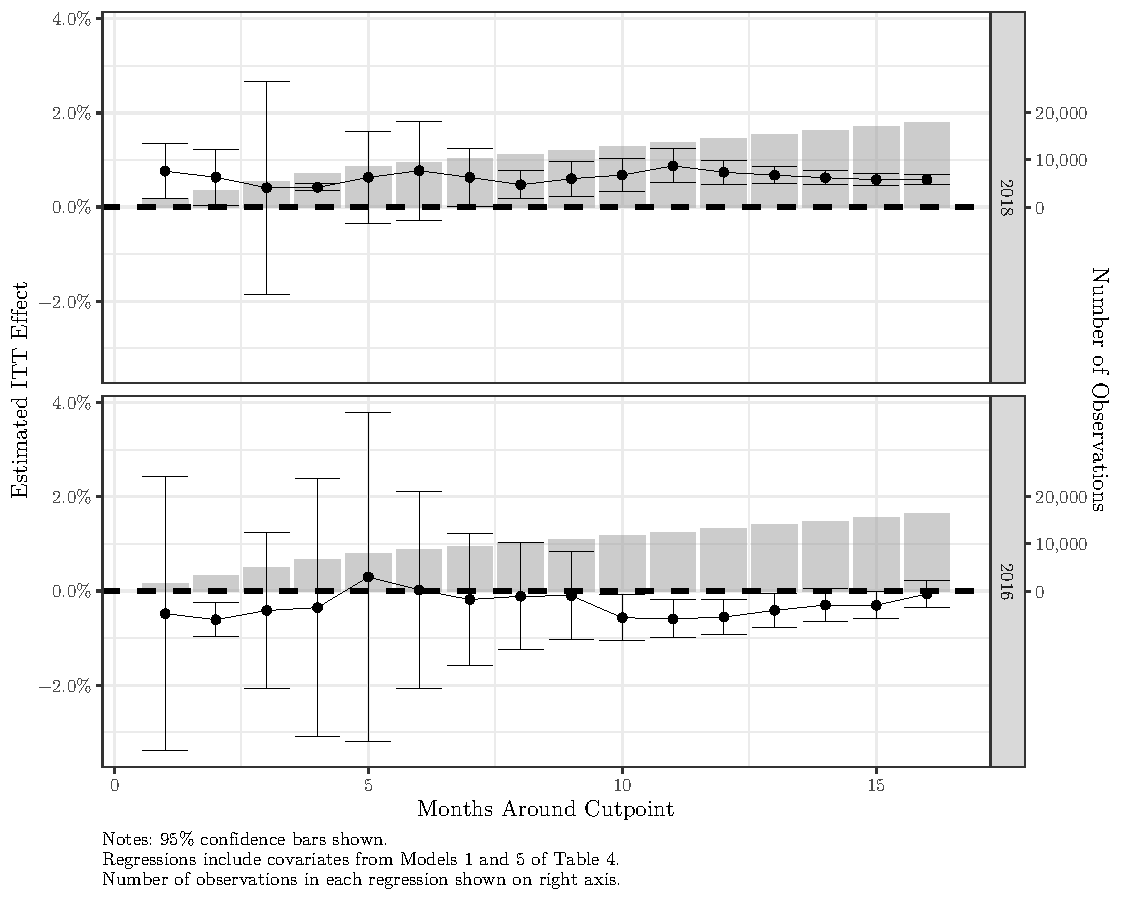
\includegraphics{rewrite_files/figure-latex/sensitivity-1} 

}

\caption{\label{fig:sens}Estimated Treatment Effect by Window Size}\label{fig:sensitivity}
\end{figure}

Although a small handful of the windows in the 2018 regressions are statistically nonsignificant, the size of the estimated treatment effect is stable and significant at the 95\% level in 13 of the 16 models. The estimated effect in the placebo regressions, on the other hand, are consistently nonsignificant or negative. This means that voters discharged in the summer before an election are perhaps \emph{less} likely to vote --- implying that our estimated effect of the executive order is perhaps somewhat conservative.

\hypertarget{racial-variation}{%
\subsection*{Racial Variation}\label{racial-variation}}
\addcontentsline{toc}{subsection}{Racial Variation}

Although these models demonstrate that rights restoration had a generally positive effect on participation in the 2018 election, the models hide substantial variation between races. Table \ref{tab:racevar} re-estimates Model 3 from Table \ref{tab:to-18-logit}, but now interacts the treatment variable with a dummy variable indicating that a former parolee was Black. As before, robust standard errors are clustered by treatment assignment group.

\begin{singlespace}

\input{"../../temp/table5.tex"}
\end{singlespace}

The estimated treatment effect for non-Black voters in Table \ref{tab:racevar} is 1.0 percentage points, though the interaction effect --- \emph{Black × D(Discharged After EO 181)} --- is negative 0.8 percentage points. The executive order was apparently substantially more effective at boosting turnout for non-Black former parolees than Black parolees. This appears to have had a leveling effect: although Black former parolees in the control group turned out at higher rates than non-Black parolees in that group, the turnout rate among Black and non-Black voters in the ITT group in 2018 was virtually identical, as shown in Table \ref{tab:re}.

\begin{singlespace}

\input{"../../temp/table_whatever3.tex"}
\end{singlespace}

\hypertarget{instrumental-variables-approach}{%
\subsection*{Instrumental Variables Approach}\label{instrumental-variables-approach}}
\addcontentsline{toc}{subsection}{Instrumental Variables Approach}

The analyses in the previous section indicate that executive order was successful at increasing turnout among formerly incarcerated individuals as a group. They do not, however, provide us an estimate of the effect of rights restoration prior to parole discharge on the specific individuals who were eligible for treatment. To answer this question, we must specifically control for whether an individual actually had his rights restored before he was discharged from parole --- not simply whether he was discharged after the policy change. Because our ITT pool in the previous section include individuals not eligible for treatment, we expect that the ITT effect will be lower than the treatment effect on the treated individuals. We consider individuals whose rights were in fact restored prior to discharge from parole ``compliers.''

Two-stage least squares models allow us to leverage the random assignment to treatment to identify the complier average causal effect (CACE). To use assignment to treatment as an instrument for compliance, assignment to treatment group must be uncorrelated with the outcome variable except via treatment (Angrist, Imbens, and Rubin \protect\hyperlink{ref-Angrist1996}{1996}). In other words, we can only uncover the CACE in this setup if, in the absence of the policy change, individuals discharged from parole before and after May 18 would have voted at the same rate in 2018. The nonsignificance of the coefficients \emph{Days off Parole} in Tables \ref{tab:to-18-logit-short} and \ref{tab:to-18-logit} indicate that this condition is met.

Table \ref{tab:iv-tab} presents the results of the two-stage least squares regression. Model 1 includes just the dummy for whether an individual's rights were restored (instrumented by treatment assignment) while Model 2 includes the additional covariates from past specifications. As before, robust standard errors are clustered by treatment assignment group.

\begin{singlespace}

\input{"../../temp/table6.tex"}
\end{singlespace}

The two-stage least squares approach indicates that the CACE was roughly 0.9 percentage points. Because overall turnout for individuals whose rights were restored was 3.2 percent, this implies that rights restoration prior to discharge from parole increased turnout by 39 percent.

\hypertarget{discussion}{%
\subsection*{Discussion}\label{discussion}}
\addcontentsline{toc}{subsection}{Discussion}

Restoring voting rights to individuals on parole is an important step toward undermining the disenfranchisement (both \emph{de jure} and \emph{de facto}) of communities of color disproportionately caught up in the criminal justice system. Prior to New York's Executive Order 181, parolees were required to wait until they finished their parole term to register to vote. That changed in 2018. On October 12\textsuperscript{th} --- the registration deadline for the 2018 midterms --- there were 21,863 active parolees whose voting rights had been restored. Without the executive order, every single one of these individuals would have been barred from participating. Though turnout among this group was low (just 832, or 3.81 percent, of these individuals successfully cast a ballot), their re-enfranchisement marks an important milestone for New York State.

As this analysis demonstrates, however, the impact of Executive Order 181 was not limited only to the individuals who would have been disenfranchised in its absence. In the case of New York State, rights restoration prior to discharge from parole is successful at boosting post-supervision participation rates. In this project we estimate that overall turnout among formerly disenfranchised individuals increased by about 0.6 percentage points (or 29 percent), and that individuals whose rights were restored saw turnout about 0.9 percentage points (or 39 percent) above where it would have been otherwise. Although the absolute impact of the policy change is small, it is meaningful given the low turnout among these individuals.

The mechanism through which the rules change increased turnout among these individuals is not clear, and deserves futher study. Weaver and Lerman (\protect\hyperlink{ref-Weaver2010}{2010}) argues that contact with the criminal justice system restructures how individuals understand their relationship with the government and sours their desire to participate. Automatic voting rights restoration upon the completion of a sentence likely does little to combat these negative perceptions of the government. On the other hand, a parolee whose parole officer actively encourages them to register and participate may believe that the state is interested in their political participation. Such interactions may undo some of the negative socialization identified by Weaver and Lerman (\protect\hyperlink{ref-Weaver2010}{2010}).

It could also be a story of better information. As Meredith and Morse (\protect\hyperlink{ref-Meredith2015}{2015}) and Gerber et al. (\protect\hyperlink{ref-Gerber2015}{2015}) show, reminding formerly disenfranchised individuals of their restored voting rights can increase their participation (but see Meredith and Morse (\protect\hyperlink{ref-Meredith2013}{2013})). Research such as Manza and Uggen (\protect\hyperlink{ref-locked_out}{2008}) further demonstrates that many formerly incarcerated individuals wrongly believe that they are ineligible to participate. When a parolee has her voting rights restored prior to discharge --- and when her parole officer is required to inform her of that fact --- she is far more likely to be confident in her voting eligibility. Of course, even voters in the control group were receiving notification of their eligibility through the mail. If the full scope of the causal effect of Executive Order 181 is informational, it is clear that information is communicated far more effectively through in-person meetings. In reality, the executive order's success at boosting turnout likely operated through multiple mechanisms.

Troublingly, the effect of pre-discharge rights restoration seems to vary based on parolees' race. This discrepancy could be caused by a number of different factors. Firstly, Black and white individuals on parole might differ in meaningful ways that impact the successfulness of the intervention. As discussed above, Black participation among individuals discharged from parole prior to the executive order voted at significantly higher rates in 2018. The intervention was likely successful for parolees who would not have voted otherwise, but needed only a small encouragement. It may be that fewer Black former parolees are susceptible to small encouragements: they may separate more cleanly into voters and nonvoters, with fewer individuals susceptible to parole officer encouragement.

We cannot, however, rule out the possibility that racial bias among parole officers plays some role in the effectiveness of the intervention. Although parole officers may not be overtly or consciously biased toward their parolees, such bias is possible. Although there is limited literature examining racial variation in parolees' perceptions of their parole officers, there is some evidence that Black prisoners report worse inmate-staff relationships than white prisoners (Hemmens and Marquart \protect\hyperlink{ref-Hemmens2000}{2000}). Moreover, recent research indicates that street-level bureaucrats may exhibit some racial bias in the services they provide. White, Nathan, and Faller (\protect\hyperlink{ref-White2015}{2015}), for instance, shows that local election administrators are less likely to respond to email questions from Latino aliases than non-Latino white aliases. There is also evidence that politicians are less likely to respond to requests from constituents of different races (Butler and Broockman \protect\hyperlink{ref-Butler2011}{2011}), and that public housing officials respond less to inquiries from Latinos (Einstein and Glick \protect\hyperlink{ref-Einstein2017}{2017}).

Parole officers may more enthusiastically encourage white parolees to register to vote and cast a ballot. This variation in encouragement would not necessarily be indicative of racial animus: it could arise from a parole officer's expectations about a parolee's political preferences. Officers are likely to provide greater encouragement to parolees they perceive to have similar political preferences. In the case of former parolees in New York State, race does serve as an effective proxy for partisanship: 82.5 percent of Black individuals discharged from parole since 2012 who participated in the 2018 election were registered Democrats; just 31.2 percent of such white individuals were registered Democrats. Ultimately, the data at hand cannot answer why the intervention succeeded at raising turnout only among white former parolees; future research must investigate why this is the case.

Re-enfranchising voters while they are still under formal supervision is obviously beneficial to the individuals who are on parole on election day; such policies allow them to make their voices heard. The case of Executive Order 181 also indicates that restoring voting rights prior to parole discharge has further benefits. In 2018, it increased turnout among individuals who were formally discharged from parole prior to the registration deadline, and therefore would have been eligible to vote even if their rights were not restored until the completion of their sentence. This is encouraging, demonstrating that the state has a unique opportunity to shape the future participation of individuals who are currently under their supervision. By restoring voting rights before individuals have completed their sentence, and by requiring parole officers to inform their parolees of their voting rights, the state can increase the political participation of a group of often-marginalized individuals, thereby increasing the democratic representation of our elections. Nevertheless, the success of the executive order is tempered by the racially disparate effects.

\newpage

\hypertarget{references}{%
\section*{References}\label{references}}
\addcontentsline{toc}{section}{References}

\hypertarget{refs}{}
\begin{cslreferences}
\leavevmode\hypertarget{ref-Angrist1996}{}%
Angrist, Joshua D., Guido W. Imbens, and Donald B. Rubin. 1996. ``Identification of Causal Effects Using Instrumental Variables.'' \emph{Journal of the American Statistical Association} 91 (434): 444--55. \url{https://doi.org/10.1080/01621459.1996.10476902}.

\leavevmode\hypertarget{ref-Angrist2008}{}%
Angrist, Joshua D., and Jörn-Steffen Pischke. 2008. \emph{Mostly Harmless Econometrics: An Empiricist's Companion}. Princeton University Press. \url{https://doi.org/10.2307/j.ctvcm4j72}.

\leavevmode\hypertarget{ref-Ansolabehere1999}{}%
Ansolabehere, Stephen D., Shanto Iyengar, and Adam Simon. 1999. ``Replicating Experiments Using Aggregate and Survey Data: The Case of Negative Advertising and Turnout.'' \emph{American Political Science Review} 93 (4): 901--9. \url{https://doi.org/10.2307/2586120}.

\leavevmode\hypertarget{ref-Burch2011}{}%
Burch, Traci. 2011. ``Turnout and Party Registration Among Criminal Offenders in the 2008 General Election.'' \emph{Law \& Society Review} 45 (3): 699--730. \url{https://doi.org/10.1111/j.1540-5893.2011.00448.x}.

\leavevmode\hypertarget{ref-Butler2011}{}%
Butler, Daniel M., and David E. Broockman. 2011. ``Do Politicians Racially Discriminate Against Constituents? A Field Experiment on State Legislators.'' \emph{American Journal of Political Science} 55 (3): 463--77. \url{https://doi.org/10.1111/j.1540-5907.2011.00515.x}.

\leavevmode\hypertarget{ref-Drucker2005}{}%
Drucker, Ernest, and Ricardo Barreras. 2005. ``Studies of Voting Behavior and Felony Disenfranchisement Among Individuals in the Criminal Justice System in New York, Connecticut, and Ohio.'' Research report. The Sentencing Project. \url{https://www.prisonpolicy.\%20org/scans/sp/fd_studiesvotingbehavior.pdf}.

\leavevmode\hypertarget{ref-Einstein2017}{}%
Einstein, Katherine Levine, and David M. Glick. 2017. ``Does Race Affect Access to Government Services? An Experiment Exploring Street-Level Bureaucrats and Access to Public Housing.'' \emph{American Journal of Political Science} 61 (1): 100--116. \url{https://doi.org/10.1111/ajps.12252}.

\leavevmode\hypertarget{ref-Gerber2000}{}%
Gerber, Alan S., and Donald P. Green. 2000. ``The Effects of Canvassing, Telephone Calls, and Direct Mail on Voter Turnout: A Field Experiment.'' \emph{American Political Science Review} 94 (3): 653--63. \url{https://doi.org/10.2307/2585837}.

\leavevmode\hypertarget{ref-Gerber2015}{}%
Gerber, Alan S., Gregory A. Huber, Marc Meredith, Daniel R. Biggers, and David J. Hendry. 2015. ``Can Incarcerated Felons Be (Re)Integrated into the Political System? Results from a Field Experiment.'' \emph{American Journal of Political Science} 59 (4): 912--26. \url{https://doi.org/10.1111/ajps.12166}.

\leavevmode\hypertarget{ref-Gerber2017}{}%
---------. 2017. ``Does Incarceration Reduce Voting? Evidence About the Political Consequences of Spending Time in Prison.'' \emph{The Journal of Politics} 79 (4): 1130--46. \url{https://doi.org/10.1086/692670}.

\leavevmode\hypertarget{ref-Hemmens2000}{}%
Hemmens, Craig, and James W. Marquart. 2000. ``Friend or Foe? Race, Age, and Inmate Perceptions of Inmate-Staff Relations.'' \emph{Journal of Criminal Justice} 28 (4): 297--312. \url{https://doi.org/10.1016/S0047-2352(00)00044-1}.

\leavevmode\hypertarget{ref-bcj_laws}{}%
Justice, Brennan Center for. 2019. ``Criminal Disenfranchisement Laws Across the United States.'' May 30, 2019. \url{https://www.brennancenter.org/our-work/research-reports/criminal-disenfranchisement-laws-across-united-states}.

\leavevmode\hypertarget{ref-Lassen2004}{}%
Lassen, David Dreyer. 2004. ``The Effect of Information on Voter Turnout: Evidence from a Natural Experiment.'' SSRN Scholarly Paper ID 475821. Rochester, NY: Social Science Research Network. \url{https://papers.ssrn.com/abstract=475821}.

\leavevmode\hypertarget{ref-Lerman2014}{}%
Lerman, Amy E., and Vesla M. Weaver. 2014. \emph{Arresting Citizenship: The Democratic Consequences of American Crime Control}. Chicago Studies in American Politics. Chicago ; London: The University of Chicago Press.

\leavevmode\hypertarget{ref-locked_out}{}%
Manza, Jeff, and Christopher Uggen. 2008. \emph{Locked Out: Felon Disenfranchisement and American Democracy}. Studies in Crime and Public Policy. New York: Oxford University Press.

\leavevmode\hypertarget{ref-Meredith2013}{}%
Meredith, Marc, and Michael Morse. 2013. ``Do Voting Rights Notification Laws Increase Ex-Felon Turnout?:'' \emph{The ANNALS of the American Academy of Political and Social Science}, November. \url{https://doi.org/10.1177/0002716213502931}.

\leavevmode\hypertarget{ref-Meredith2015}{}%
---------. 2015. ``The Politics of the Restoration of Ex-Felon Voting Rights: The Case of Iowa.'' \emph{Quarterly Journal of Political Science} 10 (1): 41--100. \url{https://doi.org/10.1561/100.00013026}.

\leavevmode\hypertarget{ref-Milligan2004}{}%
Milligan, Kevin, Enrico Moretti, and Philip Oreopoulos. 2004. ``Does Education Improve Citizenship? Evidence from the United States and the United Kingdom.'' \emph{Journal of Public Economics} 88 (9): 1667--95. \url{https://doi.org/10.1016/j.jpubeco.2003.10.005}.

\leavevmode\hypertarget{ref-Sondheimer2010}{}%
Sondheimer, Rachel Milstein, and Donald P. Green. 2010. ``Using Experiments to Estimate the Effects of Education on Voter Turnout.'' \emph{American Journal of Political Science} 54 (1): 174--89. \url{https://doi.org/10.1111/j.1540-5907.2009.00425.x}.

\leavevmode\hypertarget{ref-sentencing_2016}{}%
Uggen, Christopher, Ryan Larson, and Sarah Shannon. 2016. ``6 Million Lost Voters: State-Level Estimates of Felony Disenfranchisement, 2016.'' Research report. The Sentencing Project. \url{https://www.sentencingproject.org/publications/6-million-lost-voters-state-level-estimates-felony-disenfranchisement-2016/}.

\leavevmode\hypertarget{ref-Weaver2010}{}%
Weaver, Vesla M., and Amy E. Lerman. 2010. ``Political Consequences of the Carceral State.'' \emph{American Political Science Review} 104 (4): 817--33. \url{https://doi.org/10.1017/S0003055410000456}.

\leavevmode\hypertarget{ref-White2019}{}%
White, Ariel. 2019. ``Misdemeanor Disenfranchisement? The Demobilizing Effects of Brief Jail Spells on Potential Voters.'' \emph{American Political Science Review} 113 (2): 311--24. \url{https://doi.org/10.1017/S000305541800093X}.

\leavevmode\hypertarget{ref-White2015}{}%
White, Ariel R., Noah L. Nathan, and Julie K. Faller. 2015. ``What Do I Need to Vote? Bureaucratic Discretion and Discrimination by Local Election Officials.'' \emph{American Political Science Review} 109 (1): 129--42. \url{https://doi.org/10.1017/S0003055414000562}.
\end{cslreferences}

\end{document}
